\subsection{Grid generation for tokamak edge plasma simulations}

Tokamak boundary and divertor plasma modeling relies heavily on edge
transport modeling codes such as UEDGE \cite{Rognlien1999}, SOLPS
\cite{Wiesen2015}, EDGE2D \cite{Simonini1994}, just to mention a few
major ones. These codes are similar in many ways; they all solve the
time-evolution fluid equations for toroidally-symmetric, collisional
plasma based on the Braginskii equations, using ad-hoc radial
transport coefficients.The simulations are carried out in the actual
geometry of a modeled tokamak, to account for details of magnetic
field geometry and plasma-facing components.


Computational grids for tokamak boundary plasma modeling are usually
chosen to follow the magnetic flux surfaces, to avoid numerical
pollution caused by the extreme anisotropy of plasma transport along
and across the magnetic field \cite{Umansky2005}. Thus the
computational grid has to follow the underlying magnetic field, and
with one or several X-points present in the simulation domain the grid
topology can become highly nontrivial.

There are several grid generators for tokamak edge plasma region
currently in use. These are sufficient in most cases for modeling
single-null and double-null configurations. However modeling of
advanced divertors may require incorporating secondary X-points in the
divertor region, and grid generators currently in use for UEDGE and
other tokamak edge transport codes, e.g., CARRE \cite{Marchand1996},
are not inherently designed to produce computational grids for general
configurations containing more than one x-point at arbitrary locations
in the domain.\\ \indent

% The simplest divertor configuration consists of a single x-point (primary x-point) in the $(r,z)$ plane of our toroidally symmetric tokamak. Depending on the case of interest, the primary x-point can be located anywhere in the $(r,z)$ plane. We refer to these cases as with a single x-point as ``single-null" (SNL) configurations, and further classify them as ``lower single-null" (LSN) or ``upper single-null" (USN) configurations depending on which side of the horizontal-midplane intersecting the magnetic axis we find the x-point resides in. The primary x-point is significant in SNL cases as it corresponds to the magnetic separatrix which divides the domain into regions \cite{LLNL-TR-731515} commonly referred to in practice as the ``scrape-off layer" (SOL), ``private-flux region" (PF), and ``core-plasma region" (CORE). 
%<<<<<<< HEAD

One should note that in tokamak boundary plasma literature it is
common to refer to refer to ``inner'' and ``outer'' target plate, and
``lower'' and ``upper'' X-point. However, in general such nomenclature
can be misleading (for example, an X-point can be placed at the outer
midplane). For that reason INGRID uses its invariant notation, as
discussed further.

%In addition to provided names to these regions of interest for SNL
%cases, a notion of ``inner" and ``outer" is often used for regions
%(e.g. ``inner SOL", ``outer SOL") and target plates (e.g. ``inner
%target plate", ``outer target plate"). One can go even further and
%introduce notions of ``top`` and ``bottom" in order to define regions
%such as ``inner core top" and ``outer SOL bottom". This nomenclature
%works quite nicely for the user when considering LSN and USN
%individually, but proves to be sub-optimal when generalizing a grid
%generator to internally treat both as the general SNL case (LSN and
%USN are topologically equivalent). \\
%

%\indent For example, the notion of ``inner" and ``outer" is not
%consistent when comparing even the simplest of
%divertor-configurations/magnetic-topologies: the LSN to USN. We find
%that ``inner" and ``outer" are reflected about the vertical line
%intersecting the magnetic axis. Similarly, our notions of ``top" and
%``bottom" are also reflected about the horizontal line intersecting
%the magnetic axis. These exceptions add complexity to a grid
%generator's internals. Going further, one can see this notion of
%``inner" and ``outer" breaks down when considering the case when the
%x-point lies on the horizontal line through the magnetic-axis. Issues
%such as those mentioned above can easily result in added project
%complexity that the user may need to directly control.\\

\indent Immediately we see that if we are to design a grid generator
capable of handling x-points anywhere in the computational domain,
then we need to adopt a convention that is consistent among all
magnetic topologies of interest. This convention must also allow us to
partition the domain so that we can employ a ``divide and conquer"
strategy to obtaining a grid. We will discuss the INGRID method of
doing so in later sections.  To resolve this short-coming found in
past grid generators, we present INGRID: a Python based, interactive,
grid generator for edge plasma modeling that is currently capable of
handling up to two x-points anywhere in the computational
domain. INGRID provides a robust set of tools such as an easy to use
GUI intended for users of all levels. By internally handling the
challenges that typically arise with generating grids, INGRID can
indeed improve efficiency in a user's workflow for edge-plasma
modeling. Our INGRID algorithm's inspiration was drawn from an older
IDL-based project GINGRED \cite{izacard_umansky} where the ``divide
and conquer'' strategy for grid generation was first tried. A
motivating factor for implementing INGRID was using an open-source
language such as Python, taking advantage of its numerical and
graphical libraries.


%Although GINGRED
%provides the ability to generate grids for the configurations
%mentioned above, GINGRED has short-comings that deemed the development
%of INGRID necessary.\\

%
%\indent First, GINGRED's lack of an interactive experience limited the
%user's ability to debug/troubleshoot grid generation for error-prone
%cases. We will see that INGRID provides both an interactive workflow,
%and a modular approach to grid generation that allows users to catch
%and resolve errors on the fly. Second, GINGRED's implementation in IDL
%requires users to have access to an IDL license. This limit is one
%motivating factor for implementing INGRID an open-source language such
%as Python. Finally, GINGRED's software design pattern does not easily
%allow for the introduction of new divertor configurations and grid
%generation features of interest. INGRID heavily utilizes the
%object-oriented nature of Python for both project modularity and
%functionality.\\
%
\indent Many corner cases in tokamak edge grid generation are easier
to debug using an interactive graphical environment. Because of this,
we provide users of INGRID the ability to produce grids via a
parameter file driven GUI (in addition to direct access to the INGRID
Python package). This file allows the user to specify settings such as
paths to relevant data files, inform INGRID how many x-points to
anticipate, customize integrator settings, and fine-tune a resultant
grid. This YAML formatted parameter file allows the user to guide the
the internal INGRID algorithm at all stages of the grid generation
process and serves as the heart of the interactive GUI experience. We
will discuss this workflow in detail later in the report.\\
%
\indent When considering the idea of topological equivalences of
magnetic topologies, we naturally begin to consider when particular
magnetic topologies are not equivalent. The INGRID algorithm begins by
differentiating magnetic topologies based off the number of x-points
being taken into consideration. Since the current release of INGRID
supports up to two x-points in the computational domain, we will only
consider the SNL and DNL (double-null/two x-points) trees shown in
figure \ref{fig:config_group}. The inclusion of additional x-points in
the domain can easily follow from this proposed framework. \\
%
\indent From the tree diagram, it becomes clear that an
object-oriented design pattern could be utilized to design a modular
grid generator with magnetic topologies defined by their number of
x-points being their own classes. For special instances of cases
(i.e. LSN and USN), inheritance of a parent class is a natural
choice. The remaining challenge is to devise an identification scheme
that can discern individual magnetic topologies beyond that of the
number of x-points so that the appropriate magnetic topology is
instantiated.\\
%
\indent Before diving into the details of INGRID's topology
identification scheme, we will revisit the idea of domain partitioning
mentioned earlier and discuss how INGRID does so. We will fing this
domain partitioning plays a critical role in both INGRID's grid
generation and identification scheme for the various divertor
configurations.

%%%-move the figure to figures.tex
%\begin{figure}
%    \centering
%    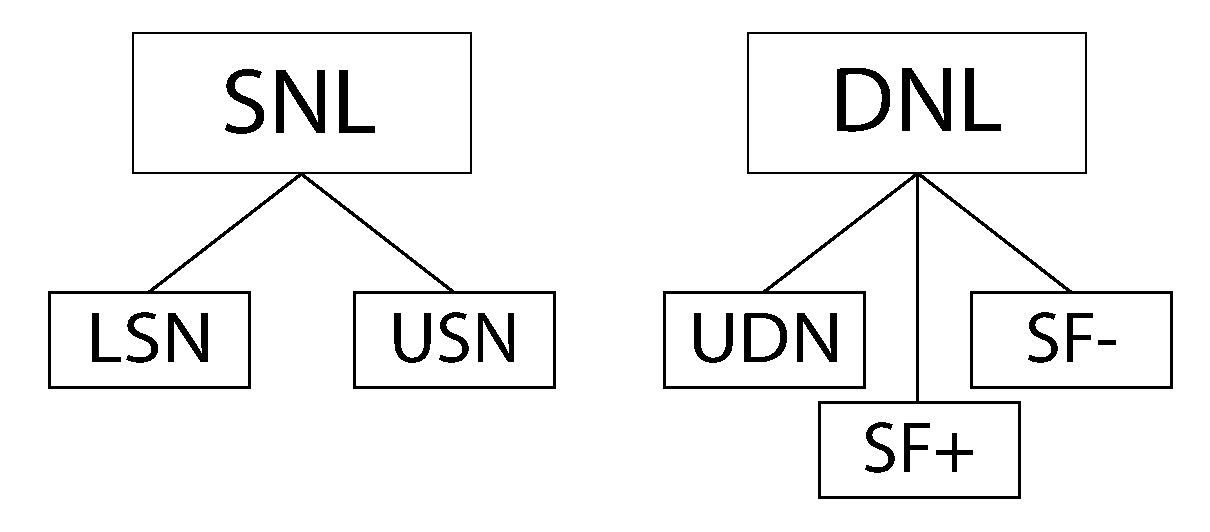
\includegraphics[width=\linewidth]{figures/config_group.pdf}
%    \caption{Categorizing magnetic topologies by number of x-points induces a natural design% pattern for a grid generator.}
%    \label{fig:config_group}
%\end{figure}
%=======

In addition to provided names to these regions of interest for SNL cases, a notion of ``inner" and ``outer" is often used for regions (e.g. ``inner SOL", ``outer SOL") and target plates (e.g. ``inner target plate", ``outer target plate"). One can go even further and introduce notions of ``top`` and ``bottom" in order to define regions such as ``inner core top" and ``outer SOL bottom". This nomenclature works quite nicely for the user when considering LSN and USN individually, but proves to be sub-optimal when generalizing a grid generator to internally treat both as the general SNL case (LSN and USN are topologically equivalent). \\ \indent
For example, the notion of ``inner" and ``outer" is not consistent when comparing even the simplest of divertor-configurations/magnetic-topologies: the LSN to USN. We find that ``inner" and ``outer" are reflected about the vertical line intersecting the magnetic axis. Similarly, our notions of ``top" and ``bottom" are also reflected about the horizontal line intersecting the magnetic axis. These exceptions add complexity to a grid generator's internals. Going further, one can see this notion of ``inner" and ``outer" breaks down when considering the case when the x-point lies on the horizontal line through the magnetic-axis. Issues such as those mentioned above can easily result in added project complexity that the user may need to directly control.\\ \indent
Immediately we see that if we are to design a grid generator capable of handling x-points anywhere in the computational domain, then we need to adopt a convention that is consistent among all magnetic topologies of interest. This convention must also allow us to partition the domain so that we can employ a ``divide and conquer" strategy to obtaining a grid. We will discuss the INGRID method of doing so in later sections.
To resolve this short-coming found in past grid generators, we present INGRID: a Python based, interactive, grid generator for edge plasma modeling that is currently capable of handling up to two x-points anywhere in the computational domain. INGRID provides a robust set of tools such as an easy to use GUI intended for users of all levels. By internally handling the challenges that typically arise with generating grids, INGRID can indeed improve efficiency in a user's workflow for edge-plasma modeling. Our INGRID algorithm's inspiration was drawn from the IDL based project GINGRED \cite{izacard_umansky}. Although GINGRED provides the ability to generate grids for the configurations mentioned above, GINGRED has short-comings that deemed the development of INGRID necessary.\\
\indent
First, GINGRED's lack of an interactive experience limited the user's ability to debug/troubleshoot grid generation for error-prone cases. We will see that INGRID provides both an interactive workflow, and a modular approach to grid generation that allows users to catch and resolve errors on the fly. Second, GINGRED's implementation in IDL requires users to have access to an IDL license. This limit is one motivating factor for implementing INGRID an open-source language such as Python. Finally, GINGRED's software design pattern does not easily allow for the introduction of new divertor configurations and grid generation features of interest. INGRID heavily utilizes the object-oriented nature of Python for both project modularity and functionality.\\ \indent
Many corner cases in tokamak edge grid generation are easier to debug using an interactive graphical environment. Because of this, we provide users of INGRID the ability to produce grids via a parameter file driven GUI (in addition to direct access to the INGRID Python package). This file allows the user to specify settings such as paths to relevant data files, inform INGRID how many x-points to anticipate, customize integrator settings, and fine-tune a resultant grid. This YAML formatted parameter file allows the user to guide the the internal INGRID algorithm at all stages of the grid generation process and serves as the heart of the interactive GUI experience. We will discuss this workflow in detail later in the report.\\
\indent
When considering the idea of topological equivalences of magnetic topologies, we naturally begin to consider when particular magnetic topologies are not equivalent. The INGRID algorithm begins by differentiating magnetic topologies based off the number of x-points being taken into consideration. Since the current release of INGRID supports up to two x-points in the computational domain, we will only consider the SNL and DNL (double-null/two x-points) trees shown in figure \ref{fig:config_group}. The inclusion of additional x-points in the domain can easily follow from this proposed framework. \\ \indent
From the tree diagram, it becomes clear that an object-oriented design pattern could be utilized to design a modular grid generator with magnetic topologies defined by their number of x-points being their own classes. For special instances of cases (i.e. LSN and USN), inheritance of a parent class is a natural choice. The remaining challenge is to devise an identification scheme that can discern individual magnetic topologies beyond that of the number of x-points so that the appropriate magnetic topology is instantiated.\\
Before diving into the details of INGRID's topology identification scheme, we will revisit the idea of domain partitioning mentioned earlier and discuss how INGRID does so. We will fing this domain partitioning plays a critical role in both INGRID's grid generation and identification scheme for the various divertor configurations.
>>>>>>> 8d3c7bf5f9747ddd5d01de38118b61fd1a87cae6
